\section{Escrevendo um gramática}

\begin{frame}[fragile]{Expressões regulares vs. gramáticas livres de contexto}

    \begin{itemize}
        \item Qualquer construção que pode ser descrita por uma expressão regular pode ser descrita por uma gramática
        \pause

        \item A recíproca nem sempre é verdadeira
        \pause

        \item Por exemplo, a expressão regular $(a\ |\ b)^*abb$ e a gramática
        \[
            \begin{array}{l}
                A_0\to aA_0\ |\ bA_0\ |\ aA_1 \\
                A_1\to bA_2 \\
                A_2\to bA_3 \\
                A_3\to \code{apl}{∊}
            \end{array}
        \]
        descrevem a mesma linguagem
        \pause

        \item É possível converter automaticamente um autômatico finito não-determinístico em uma gramática que gere a mesma linguagem do AFN
    \end{itemize}

\end{frame}

\begin{frame}[fragile]{Algoritmo de conversão de um AFN para uma gramática livre de contexto}

    \begin{algorithmic}[1]
        \Require{um AFN}
        \Ensure{uma gramática livre de contexto} 

        \For{cada estado $i$ do AFN}
            \State{crie um símbolo não-terminal $A_i$ da gramática}
            \If{o estado $i$ possui um transição para o estado $j$ com rótulo $a$}
                \State{introduza a produção $A_i\to aA_j$ na gramática}
            \ElsIf{o estado $i$ possui um transição para o estado $j$ com rótulo \code{apl}{∊}}
                \State{introduza a produção $A_i\to A_j$ na gramática}
            \EndIf
            \If{o estado $i$ é um estado de aceitação}
                \State{introduza a produção $A_i\to \code{apl}{∊}$ na gramática}
            \ElsIf{o estado $i$ é o estado de partida}
                \State{torne o estado $A_i$ o símbolo de partida da gramática}
            \EndIf
        \EndFor
    \end{algorithmic}

\end{frame}

\begin{frame}[fragile]{Razões para o uso de expressões regulares para definir a estrutura léxica}

    \begin{enumerate}
        \item As regras léxicas de uma linguagem geralmente são simples, sendo as expressões regulares suficientes para descrevê-las
        \pause

        \item As expressões regulares, em geral, descrevem os tokens da linguagem de forma mais concisa e clara do que as gramáticas livres de contexto
        \pause

        \item É possível gerar analisadores léxicos mais eficientes a partir de expressões regulares do que a partir de gramáticas arbitrárias
        \pause

        \item A separação da estrutura léxica da estrutura sintática permite a modularização da interface de vanguarda
    \end{enumerate}

\end{frame}

\begin{frame}[fragile]{Verificando a linguagem gerada por uma gramática}

    \begin{itemize}
        \item A prova que uma gramática $G$ gera uma linguagem $L(G)$ é feita em duas etapas:
        \pause
        \begin{enumerate}
            \item mostrar que cada cadeia gerada por $G$ está em $L(G)$
            \pause

            \item mostrar que cada cadeia em $L(G)$ pode ser gerada por $G$
        \end{enumerate}
        \pause

        \item Por exemplo, considere a gramática
        \[
            S\to (S)S\ |\ \code{apl}{∊}
        \]
        \pause

        \item Esta gramática gera todas as cadeias de parêntesis balanceadas
        \pause

        \item Para provar esta afirmação, primeiro é preciso provar que qualquer cada sentença derivável de $S$ é balanceada
        \pause

        \item Esta prova é feita por indução no número de passos da derivação
    \end{itemize}

\end{frame}

\begin{frame}[fragile]{Verificando a linguagem gerada por uma gramática}

    \begin{itemize}
        \item Em apenas um passo de derivação, a única cadeia gerada é a cadeia vazia \code{apl}{∊}, a qual é trivialmente balanceada
        \pause

        \item Suponha que qualquer derivação com menos do que $n$ passos gere uma cadeia balanceada
        \pause

        \item Uma derivação com exatamente $n$ passos tem a forma
        \[
            S\Rightarrow (S)S \overset{\scalebox{0.5}*}{\Rightarrow} (x)S \overset{\scalebox{0.5}*}{\Rightarrow} (x)y
        \]
        onde $x$ e $y$ são derivações com que $n$ passos
        \pause

        \item Pela hipótese de indução, $x$ e $y$ são balanceadas e, portanto, a derivação $S$ com exatamente $n$ passos também é balanceada
    \end{itemize}

\end{frame}

\begin{frame}[fragile]{Verificando a linguagem gerada por uma gramática}

    \begin{itemize}
        \item A prova que qualquer cadeia balanceada é derivável a partir de $S$ é feita por meio de indução no comprimento da cadeia
        \pause

        \item A menor cadeia balanceada é a cadeia vazia, que é derivável a partir de $S$ por meio da produção $S\to \code{apl}{∊}$
        \pause

        \item Suponha que todas as cadeias balanceadas com comprimento menor do que $2n$ sejam deriváveis a partir de $S$ e que $w$ seja uma cadeia balanceada de tamanho
            $2n$
        \pause

        \item Certamente $w$ inicia com um parêntesis à esquerda
        \pause

        \item Seja $(x)$ o menor prefixo de $w$ com o mesmo número de parêntesis à esquerda e à direita
        \pause

        \item Assim, $w = (x)y$, onde $x$ e $y$ são cadeias balanceadas com comprimento menor do que $2n$
        \pause

        \item Pela hipótese de indução, $x$ e $y$ são deriváveis a partir de $S$
        \pause

        \item Assim, $w$ é derivável a partir de $S$, por meio da derivação
        \[
            S\Rightarrow (S)S \overset{\scalebox{0.5}*}{\Rightarrow} (x)S \overset{\scalebox{0.5}*}{\Rightarrow} (x)y
        \]
    \end{itemize}

\end{frame}

\begin{frame}[fragile]{Eliminando a ambiguidade}

    \begin{itemize}
        \item Uma gramática pode ser reescrita para eliminar possíveis ambiguidades
        \pause

        \item Por exemplo, considere a gramática abaixo, que torna o \code{apl}{else} opcional:
        \[
            \begin{array}{rcl}
                cmd & \to & \textbf{if}\ expr\ \textbf{then}\ cmd \\
                & | & \textbf{if}\ expr\ \textbf{then}\ \textbf{else}\ cmd \\
                & | & \textbf{outro}
            \end{array}
        \]
        \pause

        \item Na gramática, \textbf{outro} significa qualquer outro enunciado
        \pause

        \item Esta gramática é ambígua: a cadeia
        \[
            \textbf{if}\ E_1\ \textbf{then if}\ E_2\ \textbf{then}\ S_1\ \textbf{else}\ S_2
        \]
        possui duas árvores gramaticais distintas
    \end{itemize}

\end{frame}

\begin{frame}[fragile]{Primeira árvore gramatical para a expressão `$\textbf{if}\ E_1\ \textbf{then if}\ E_2\ \textbf{then}\ S_1\ \textbf{else}\ S_2$'}

    \begin{figure}
        \centering

        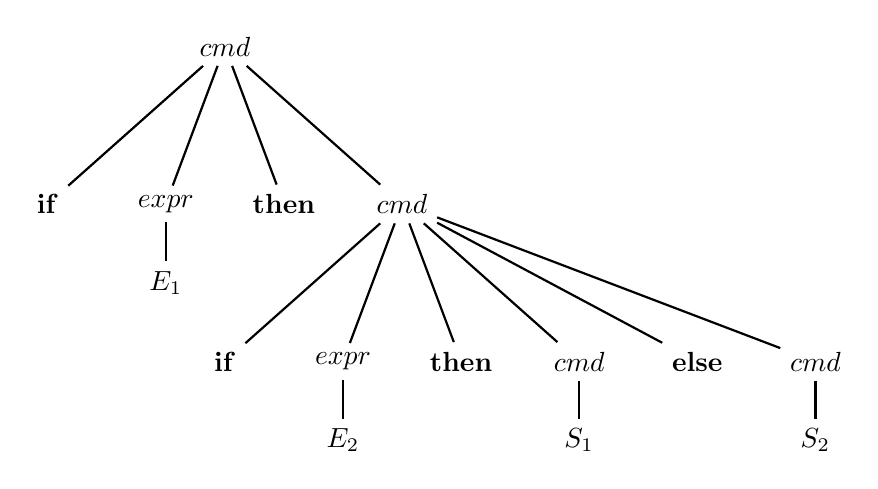
\begin{tikzpicture} 
            \node (A) at (2.25, 6) { $cmd$ };

            \node (B1) at (0, 4) { \textbf{if} };
            \node (B2) at (1.5, 4) { $expr$ };
            \node (B3) at (3, 4) { \textbf{then} };
            \node (B4) at (4.5, 4) { $cmd$ };

            \node (C0) at (1.5, 3) { $E_1$ };
            \node (C1) at (2.25, 2) { \textbf{if} };
            \node (C2) at (3.75, 2) { $expr$ };
            \node (C3) at (5.25, 2) { \textbf{then} };
            \node (C4) at (6.75, 2) { $cmd$ };
            \node (C5) at (8.25, 2) { \textbf{else} };
            \node (C6) at (9.75, 2) { $cmd$ };

            \node (D1) at (3.75, 1) { $E_2$ };
            \node (D2) at (6.75, 1) { $S_1$ };
            \node (D3) at (9.75, 1) { $S_2$ };

            \draw[thick] (A) to (B1);
            \draw[thick] (A) to (B2);
            \draw[thick] (A) to (B3);
            \draw[thick] (A) to (B4);
            \draw[thick] (B2) to (C0);
            \draw[thick] (B4) to (C1);
            \draw[thick] (B4) to (C2);
            \draw[thick] (B4) to (C3);
            \draw[thick] (B4) to (C4);
            \draw[thick] (B4) to (C5);
            \draw[thick] (B4) to (C6);

            \draw[thick] (C2) to (D1);
            \draw[thick] (C4) to (D2);
            \draw[thick] (C6) to (D3);
        \end{tikzpicture} 
    \end{figure}

\end{frame}

\begin{frame}[fragile]{Segunda árvore gramatical para a expressão `$\textbf{if}\ E_1\ \textbf{then if}\ E_2\ \textbf{then}\ S_1\ \textbf{else}\ S_2$'}

    \begin{figure}
        \centering

        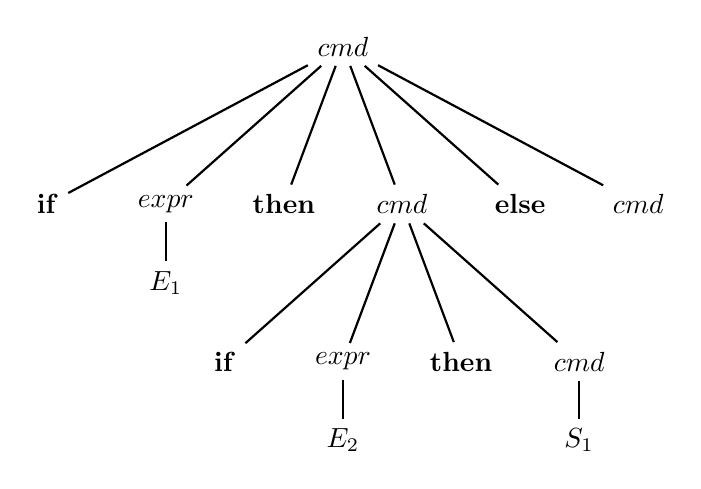
\begin{tikzpicture} 
            \node (A) at (3.75, 6) { $cmd$ };

            \node (B1) at (0, 4) { \textbf{if} };
            \node (B2) at (1.5, 4) { $expr$ };
            \node (B3) at (3, 4) { \textbf{then} };
            \node (B4) at (4.5, 4) { $cmd$ };
            \node (B5) at (6, 4) { \textbf{else} };
            \node (B6) at (7.5, 4) { $cmd$ };

            \node (C0) at (1.5, 3) { $E_1$ };
            \node (C1) at (2.25, 2) { \textbf{if} };
            \node (C2) at (3.75, 2) { $expr$ };
            \node (C3) at (5.25, 2) { \textbf{then} };
            \node (C4) at (6.75, 2) { $cmd$ };

            \node (D1) at (3.75, 1) { $E_2$ };
            \node (D2) at (6.75, 1) { $S_1$ };

            \draw[thick] (A) to (B1);
            \draw[thick] (A) to (B2);
            \draw[thick] (A) to (B3);
            \draw[thick] (A) to (B4);
            \draw[thick] (A) to (B5);
            \draw[thick] (A) to (B6);
            \draw[thick] (B2) to (C0);
            \draw[thick] (B4) to (C1);
            \draw[thick] (B4) to (C2);
            \draw[thick] (B4) to (C3);
            \draw[thick] (B4) to (C4);

            \draw[thick] (C2) to (D1);
            \draw[thick] (C4) to (D2);
        \end{tikzpicture} 
    \end{figure}

\end{frame}

\begin{frame}[fragile]{Reescrita para a eliminação da ambiguidade}

    \begin{itemize}
        \item Na maioria das linguagens, a primeira das duas árvores seria a esperada
        \pause

        \item A regra geral é associar cada \textbf{else} ao \textbf{then} anterior mais próximo ainda não associado
        \pause

        \item Para reescrita, a ideia é que um enunciado entre um \textbf{then} e um \textbf{else} precisa estar associado, isto é, não pode terminar em um
            \textbf{then} não associado a um \textbf{else}
        \pause
    \end{itemize}

    \[
        \begin{array}{rcl}
            cmd & \to & cmd\_associado \\
                & | & cmd\_nao\_associado \\
            cmd\_associado & \to & \textbf{if}\ expr\ \textbf{then}\ cmd\_associado\ \textbf{else}\ cmd\_associado \\
            & | & \textbf{outro} \\
            cmd\_nao\_associado & \to & \textbf{if}\ expr\ \textbf{then}\ cmd \\
            & | & \textbf{if}\ expr\ \textbf{then}\ cmd\_associado\ \textbf{else}\ cmd\_nao\_associado
        \end{array}
    \]
\end{frame}

\begin{frame}[fragile]{Gramáticas recursivas à esquerda}

    \begin{itemize}
        \item Uma gramática é recursiva à esquerda se possui um não-terminal $A$ tal que existe um derivação $A\overset{\scalebox{0.5}{+}}{\Rightarrow} A\alpha$
            para alguma cadeia $\alpha$
        \pause

        \item Métodos \textit{top-down} não podem processar gramáticas recursivas à esquerda, demandando uma reescrita da gramática que elimine a recursão à
        esquerda
        \pause

        \item Uma recursão simples à esquerda acontece se existe um produção $A\to A\alpha$
        \pause

        \item A recursão simples à esquerda de uma produção da forma $A\to A\alpha\ |\ \beta$ pode ser eliminada ao substituí-la pelas produções
        \[
            \begin{array}{l}
                A \to \beta A' \\
                A' \to \alpha A'\ |\ \code{apl}{∊}
            \end{array}
        \]
    \end{itemize}

\end{frame}

\begin{frame}[fragile]{Exemplo de eliminação de recursão simples à esquerda}

\[
    \begin{array}{lp{3cm}l}
        E\to E\ \code{apl}{+}\ T\ |\ T & & E\to TE' \\
        T\to T\ \code{apl}{×}\ F\ |\ F & & E'\to \code{apl}{+}\ TE'\ |\ \code{apl}{∊} \\
        F\to (E)\ |\ \textbf{id} & & T\to FT'\\
        & & T'\to \code{apl}{×}\ FT'\ |\ \code{apl}{∊} \\
        & & F\to (E)\ |\ \textbf{id}
    \end{array}
\]

\end{frame}

\begin{frame}[fragile]{Eliminação de recursão à esquerda}

    \begin{itemize}
        \item No caso geral, é possível eliminar todas as recursões simples à esquerda nas produções-$A$ de uma só vez
        \pause

        \item Primeiramente, organize todas as produções-$A$ na forma
        \[
            A\to A\alpha_1\ |\ A\alpha_2\ |\ \ldots\ |\ A\alpha_m\ |\ \beta_1\ |\ \beta_2\ |\ \ldots\ |\ \beta_n
        \]
        onde nenhum $\beta_j$ começa com um $A$
        \pause

        \item Em seguida, substitua estas produções-$A$ pelas produções
        \[
            \begin{array}{l}
                A\to \beta_1 A'\ |\ \beta_2 A'\ |\ \ldots \ |\ \beta_n A'\\
                A'\to \alpha_1  A'\ |\ \alpha_2 A'\ |\ \ldots\ |\ \alpha_m A'\ |\ \code{apl}{∊}
            \end{array}
        \]
        \pause

        \item Esta substituição elimina todas as recursões simples à esquerda de uma só vez, desde que $\alpha_i \neq \code{apl}{∊}$ para todo $i = 1, 2, \ldots, m$
        \pause

        \item Esta técnica, porém, não elimina recursões à esquerda envolvendo derivações com dois ou mais passos
    \end{itemize}

\end{frame}

\begin{frame}[fragile]{Algoritmo para eliminação de recursão à esquerda}

    \begin{algorithmic}[1]
        \Require{Uma gramática $G$ sem ciclos (isto é, produções $A\overset{\scalebox{0.5}{+}}{\Rightarrow} A$) e sem produções-\code{apl}{∊} (do tipo $A\to 
            \code{apl}{∊}$)}
        \Ensure{Uma gramática equivalente a $G$ sem recursão à esquerda}
 
        \vspace{0.2in}

        \State{Liste, em alguma ordem, os não-terminais $A_1, A_2, \ldots, A_n$}
        \For{$i\gets 1, n$}
            \For{$j\gets 1, i - 1$}
                \State{substitua cada produção $A_i\to A_j\gamma$ pelas produções $$A_i \to \delta_1\gamma \ |\ \delta_2\gamma \ |\ \ldots \ |\ \delta_k\gamma,$$ onde $A_j\to \delta_1 \ |\ \delta_2 \ |\ \ldots \ |\ \delta_k$ são todas as produções-$A_j$ atuais}
            \EndFor
            \State{elimine todas as recursões simples à esquerda nas produções-$A_i$}
        \EndFor
    \end{algorithmic} 

\end{frame}

\begin{frame}[fragile]{Exemplo de eliminação de recursão à esquerda}

    \begin{itemize}
        \item Considere a gramática
        \[
            \begin{array}{l}
                S \to Aa\ |\ b \\
                A \to Ac\ |\ Sc\ |\ \code{apl}{∊}
            \end{array}
        \]
        \pause

        \item Observe que o não-terminal $S$ é recursivo à esquerda, pois
        \[
            S \Rightarrow Aa \Rightarrow Sda
        \]
        \pause

        \item A aplicação do algoritmo de eliminação de recursão poderia não funcionar, por conta da produção-\code{apl}{∊} do não-terminal $A$, mas neste
            caso em particular o algoritmo de fato elimina a recursão
    \end{itemize}

\end{frame}

\begin{frame}[fragile]{Exemplo de eliminação de recursão à esquerda}

    \begin{itemize}
        \item Usando a ordenação $S, A$, o primeiro iteração do algoritmo não altera a gramática, uma vez que $S$ não tem recursão simples à esquerda
        \pause

        \item Na segunda iteração, as produções-$A$ que envolvem $S$ devem ser substituídas, obtendo
        \[
            A\to Ac\ |\ Aad\ |\ bd\ |\ \code{apl}{∊}
        \]
        \pause

        \item A eliminação da recursão simples à esquerda nas produções-$A$ resulta na gramática livre de recursão à esquerda
        \[
            \begin{array}{l}
                S \to Aa\ |\ b \\
                A \to bdA'\ |\ A' \\
                A' \to cA'\ |\ adA'\ |\ \code{apl}{∊}
            \end{array}
        \]
    \end{itemize}

\end{frame}

\begin{frame}[fragile]{Fatoração à esquerda}

    \begin{itemize}
        \item A fatoração à esquerda é uma técnica útil para a criação de gramáticas que beneficia a análise preditiva
        \pause

        \item A ideia central da fatoração à esquerda e evitar ambiguidades, quando duas ou mais produções tenham prefixos comuns
        \pause

        \item Por exemplo, considere as produções $A \to \alpha \beta_1\ |\ \alpha \beta_2$
        \pause

        \item Se a entrada contém uma cadeia não-vazia derivada a partir de $\alpha$, não é possível decidir, de antemão, qual das duas produções usar
        \pause

        \item A fatoração à esquerda propõe a reescrita das produções da seguinte forma, que elimina a ambiguidade
        \[
            \begin{array}{l}
                A \to \alpha A' \\
                A' \to \beta_1\ |\ \beta_2
            \end{array}
        \]
    \end{itemize}

\end{frame}

\begin{frame}[fragile]{Exemplo de fatoração à esquerda}

    \begin{itemize}
        \item Muitas linguagens permitem que o comando \textbf{if-then-else} tenha um \textbf{else} vazio:
        \[
            \begin{array}{rcl}
                cmd & \to & \textbf{if}\ expr\ \textbf{then}\ cmd\ \textbf{else}\ cmd \\ 
                & | & \textbf{if}\ expr\ \textbf{then}\ cmd
            \end{array}
        \]
        \pause

        \item Esta gramática pode ser abstraída da seguinte forma
        \[
            \begin{array}{l}
                S \to iEtS\ |\ iEtSeS\ |\ a \\
                E \to b
            \end{array}
        \]
        \pause

        \item A fatoração à esquerda esta gramática resulta em
        \[
            \begin{array}{l}
                S \to iEtSS'\ |\ a \\
                S' \to eS\ |\ \code{apl}{∊} \\
                E \to b
            \end{array}
        \]
    \end{itemize}

\end{frame}

\begin{frame}[fragile]{Exemplos de linguagens não livres de contexto}

    \begin{itemize}
        \item Considere a linguagem abstrata
        \[
            L_1 = \{ wcw\ |\ w\in (a\ |\ b)^*\}
        \]
        \pause

        \item As sentenças de $L_1$ são formada por uma cadeia $w$ de $a$'s e $b$'s, seguida de um $c$ e repetida em seguida (por exemplo, $abaabcabaab$)
        \pause

        \item É possível demostrar que a linguagem $L_1$ não é livre de contexto
        \pause

        \item Tal linguagem abstrai o problema de se verificar se um identificador ($w$) foi declarado antes de seu uso ($c$ é o que separa a declaração do
            primeiro uso)
        \pause

        \item Não sendo possível definir tal regra sintaticamente, esta verificação fica postergada para a análise semântica
    \end{itemize}

\end{frame}

\begin{frame}[fragile]{Exemplos de linguagens não livres de contexto}

    \begin{itemize}
        \item Considere a linguagem abstrata
        \[
            L_2 = \{ a^nb^mc^nd^m\ |\ n \geq 1\ \mbox{e}\ m\geq 1\}
        \]
        \pause

        \item As senteças de $L_2$ são cadeias onde o número de $a$'s coincide com o número de $c$'s, e o número de $b$'s coincide com o número de $d$'s, em ordem
            lexicográfica
        \pause

        \item $L_2$ também não é livre de contexto
        \pause

        \item Ela abstrai o problema de ser verificar se o número de parâmetros na declaração de uma função é igual ao número de parâmetros na chamada ($a^n$ e
            $b^m$ seriam as listas de parâmetros de dois procedimentos e $c^n$ e $d^n$ o número de parâmetros na chamada destes procedimentos)
    \end{itemize}

\end{frame}

\begin{frame}[fragile]{Exemplos de linguagens não livres de contexto}

    \begin{itemize}
        \item A linguagem
        \[
            L_3 = \{ a^nb^nc^n\ |\ n\geq 1\}
        \]
        também não é livre de contexto
        \pause

        \item A diferença entre uma linguagem livre de uma não-livre pode ser sutil
        \pause

        \item Por exemplo, a linguagem
        \[
            L'_1 = \{ wcw^R\ |\ w\in (a\ |\ b)^*\},
        \]
        onde $w^R$ é o reverso de $w$, é livre de contexto
        \pause

        \item Ela pode ser gerada pela gramática $S\to aSa\ |\ bSb\ |\ \code{apl}{∊}$
    \end{itemize}

\end{frame}

\begin{frame}[fragile]{Exemplos de linguagens não livres de contexto}

    \begin{itemize}
        \item A linguagem
        \[
            L'_2 = \{ a^nb^mc^md^n\ |\ n\geq 1\ \mbox{e}\ m\geq 1\}
        \]
        também é livre de contexto
        \pause

        \item A gramática abaixo gerada $L'_2$:
        \[
            \begin{array}{l}
                S \to aSd\ |\ aAd \\
                A \to bAc\ |\ bc
            \end{array}
        \]
        \pause

        \item A linguagem
        \[
            L''_2 = \{ a^nb^nc^md^m\ |\ n\geq 1\ \mbox{e}\ m\geq 1\}
        \]
        também é livre de contexto
        \pause

        \end{itemize}

\end{frame}

\begin{frame}[fragile]{Exemplos de linguagens não livres de contexto}

    \begin{itemize}
        \item Ela pode ser gerada pela gramática
        \[
            \begin{array}{l}
                S \to A\ |\ B \\
                A \to aAb\ |\ ab \\
                B \to cBd\ |\ cd
            \end{array}
        \]
        \pause

        \item Por fim, a linguagem
        \[
            L'_3 = \{ a^nb^n\ |\ n\geq 1\}
        \]
        é livre de contexto, gerada pela gramática $S\to aSb\ |\ ab$
        \pause

        \item Informalmente, pode-se afirmar que um autômato finito não pode realizar contagens e que uma gramática pode manter uma contagem de dois itens, mas
            não de três
    \end{itemize}

\end{frame}
